\documentclass[letterpaper,12pt,oneside]{book}
%\usepackage[a4paper,includeall,bindingoffset=0cm,margin=2cm,marginparsep=0cm,marginparwidth=0cm]{geometry}
%\usepackage[top=1in, left=0.9in, right=1.25in, bottom=1in]{geometry}
%\usepackage{bachelorstitlepageUNAM}
\usepackage{ragged2e}
\usepackage{times}
\usepackage{listings}
\usepackage{xcolor}
%\usepackage{background}
\usepackage[utf8]{inputenc}
\usepackage{url}
\usepackage[T1]{fontenc}
\usepackage[spanish,es-nodecimaldot,es-tabla]{babel}
\usepackage{graphicx}
\usepackage{tikz}
\usepackage{tocloft}
\graphicspath{{./figs/}}
\usepackage{setspace}
\usepackage{comment}
\usepackage{hyperref}
\urlstyle{same}
\hypersetup{
   colorlinks=true,
   urlcolor=cyan,
   linkcolor=black,
   citecolor=black,
   filecolor=magenta,
   pdftitle={Sharelatex Example},
   pdfpagemode=FullScreen,
}
\usepackage[natbibapa]{apacite}
%\usepackage[round]{natbib}

%\renewcommand\cftsecpresnum{\S}
%\renewcommand\cftsubsecpresnum{\S}

%%%%%%%%%%%%%%%%%%%%%%%%%%%%%

% Modificación de la plantilla original de esta url: 
% https://es.overleaf.com/latex/templates/tesis-unam-ingenieria-energia/kfffjrxcckdp

% Adaptada por Carlos Rodríguez Díaz para el CIC IPN.
% Cualquier sugerencia, corrección o comentario a: amnet04@gmail.com

% A continuación los comentarios de la plantilla original:

% Comparto una plantilla para la PORTADA que us\'e en mi t\'esis
% basada en el dise\~no gen\'erico que se usa en la Facultad de Ciencias
% Para usarlo \'unicamente aseg\'urate de tener la l\'inea
% \usepackage{bachelorstitlepageUNAM} y el archivo bachelorstitlepageUNAM.sty en el mismo directorio de trabajo.
% y los campos (sin signo %) :
%\author{Nombre del Alumno}
%\title{T\'itulo de la tesis}
%\faculty{Facultad}
%\degree{Grado que obtienes}
%\supervisor{ Tutor}
%\cityandyear{Ciudad y anio}
%\logouni{nombredelescudodelaunamsinespacios}
%\logofac{NombreDeLaImagenDelEscudodeTuFacultadSinEspacios}
% Para sugerencias y comentarios: DM en twitter.com/sglvgdor
% Subir\'e mas adelante la plantilla para maestr\'ia
%%%%%%%%%%%%%%%%%%%%%%%%%%%%%


\begin{document}

\frontmatter
            \begin{titlepage}
  \thispagestyle{empty}
  \begin{minipage}[c][0.17\textheight][c]{0.25\textwidth}
    \begin{center}
      
\includegraphics[ height=4cm]{Images/logo-ipn.png}
    \end{center}
  \end{minipage}
  \begin{minipage}[c][0.195\textheight][t]{0.75\textwidth}
    \begin{center}
      \vspace{0.3cm}
             {\color{red}\textsc{\large Instituto Politécnico Nacional} }\\[0.5cm]
             \vspace{0.3cm}
                    {\color{purple}\hrule height2.5pt}
                    \vspace{.2cm}
                           {\color{purple}\hrule height1pt}
                           \vspace{.8cm}
                           \textsc{Escuela Superior de Cómputo }\\[1cm] %
    \end{center}
  \end{minipage}
  \begin{minipage}[c][0.81\textheight][t]{0.25\textwidth}
    \vspace*{5mm}
    \begin{center}
      \hskip2.0mm
             {\color{red}\vrule width1pt height13cm }
             \vspace{5mm}
             \hskip2pt
                 {\color{red}\vrule width2.5pt height13cm}
                 \hskip2mm
                     {\color{red}\vrule width1pt height13cm} \\
                     \vspace{5mm}
                     
\includegraphics[height=3.0cm]{Images/CIC.png}
    \end{center}
  \end{minipage}
  \begin{minipage}[c][0.81\textheight][t]{0.75\textwidth}
    \begin{center}
      \vspace{1cm}

      {\color{red}{\large\scshape Titulo del Reporte }}\\[.2in]

      \vspace{2cm}            

      \textsc{\LARGE P\hspace{0.5cm}R\hspace{0.5cm}O\hspace{0.5cm}G\hspace{0.5cm}R\hspace{0.5cm}A\hspace{0.5cm}M\hspace{0.5cm}A\hspace{0.5cm}}\\[1cm]
      \textsc{\LARGE G\hspace{0.5cm}R\hspace{0.5cm}A\hspace{0.5cm}M\hspace{0.5cm}Á\hspace{0.5cm}T\hspace{0.5cm}I\hspace{0.5cm}C\hspace{0.5cm}A}\\[1cm]
      \textsc{\LARGE\hspace{0.5cm}A\hspace{0.5cm}M\hspace{0.5cm}B\hspace{0.5cm}I\hspace{0.5cm}G\hspace{0.5cm}U\hspace{0.5cm}A}
      \\[1cm]
      \textsc{\large que para obtener un 10 en el reporte:}\\[0.2cm]
     % \textsc{\large XXXX XXXX XXXXX}\\[0.5cm]
      
      {\color{red}\textsc{\large presenta:}}\\[0.2cm]
      \textsc{\large {Connor Urbano Mendoza}}\\[1cm]          

      \vspace{0.5cm}

      {\large\scshape 
        {\color{red}Docente:}\\[0.3cm] {Juárez Martínez Genaro}}\\[.2in]

      \vspace{1cm}

      \large{Estados Unidos Mexicanos\\ 
        Ciudad de México\\
        2023}
    \end{center}
  \end{minipage}
\end{titlepage}
%---------------------------------
\tableofcontents
\listoffigures
%\chapter{Notación}


\chapter{Introducción}
La práctica consiste en elaborar un programa para procesar una gramática no ambigua. En esta gramática, se definen dos reglas de producción:\newline
\begin{enumerate}
    \item B -> (RB | ε: Esta regla indica que el símbolo no terminal B puede ser reemplazado por la secuencia $'$(RB$'$ o puede ser eliminado, es decir, puede ser el símbolo vacío.\newline
    \item R -> ) | (RR: Esta regla indica que el símbolo no terminal R puede ser reemplazado por el símbolo $'$)$'$ o puede ser seguido por la secuencia $'$(RR$'$.\newline
\end{enumerate}

El objetivo del programa es tomar una cadena de entrada conformada por paréntesis balanceados y aplicar una derivación única y a la izquierda para obtener una cadena generada. El proceso de derivación se realiza escaneando la cadena de izquierda a derecha y aplicando las reglas de producción correspondientes.\newline

El programa debe contar con las siguientes características adicionales:\newline
\begin{enumerate}
    \item La cadena de entrada puede ser ingresada por el usuario o generada automáticamente.\newline
    \item La evaluación de la gramática debe ser impresa en pantalla y/o guardada en un archivo. Se debe indicar el símbolo que se está evaluando, la producción aplicada y la cadena generada en cada paso.\newline
    \item El programa debe ser capaz de manejar cadenas de hasta 1,000 caracteres de longitud.\newline
\end{enumerate}

Es importante seguir las condiciones de evaluación establecidas por el docente, como subir un informe en formato PDF al aula virtual, adjuntando el código fuente en LaTeX.\newline

Esta práctica se basa en conceptos de teoría de la computación, específicamente en el estudio de gramáticas formales y sus derivaciones. El propósito es aplicar estos conceptos para implementar un programa que pueda procesar y generar cadenas válidas según una gramática específica.\newline



\mainmatter
\chapter{Desarrollo}
\lstset{
    language=C,
    basicstyle=\ttfamily\small\color{black},
    numbers=left,
    numberstyle=\tiny,
    stepnumber=1,
    numbersep=8pt,
    backgroundcolor=\color{white},
    showspaces=false,
    showstringspaces=false,
    showtabs=false,
    frame=single,
    rulecolor=\color{magenta},
    tabsize=2,
    captionpos=b,
    breaklines=true,
    breakatwhitespace=false,
    title=\lstname,
    escapeinside={\%*}{*)},
    keywordstyle=\color{blue},
    commentstyle=\color{red},
    stringstyle=\color{orange},
    morecomment=[l][\color{red}]{\#},
    otherkeywords={=,!,<,>,*,+,-,&,|,^,~},
    numbers=left,                   % Coloca los números de línea a la izquierda
    numberstyle=\tiny\color{black}, % Estilo de los números de línea
    stepnumber=1,    % Incremento en el que se muestran los números de línea
    numbersep=8pt
}
\section{Análisis del problema principal}

%\begin{comment}
  %Objetivo: Explicarles a los lectores de computación que entienden
  %los lingüistas de una variación dialectal
%\end{comment}

%Citar a \cite{deSaussure1945}, Coseriu y Montes:

Para abordar este problema, se deben considerar los siguientes aspectos:\newline
\begin{enumerate}
    \item Definición de la gramática: Es necesario comprender las reglas de producción y las estructuras permitidas en la gramática no ambigua dada. En este caso, se tienen las reglas $B -> (RB | ε y R -> ) $| (RR. Estas reglas establecen cómo se pueden reemplazar los símbolos no terminales B y R.\newline

    \item Análisis de la cadena de entrada: Se debe leer la cadena de entrada proporcionada por el usuario o generada automáticamente. Es importante verificar que la cadena cumpla con las condiciones requeridas, en este caso, que esté compuesta únicamente por paréntesis balanceados.\newline
    
    \item Aplicación de las reglas de producción: Utilizando la técnica de derivación a la izquierda, se deben aplicar las reglas de producción correspondientes para generar la cadena resultante. En cada paso, se evalúa el siguiente símbolo de la cadena de entrada y se determina qué regla se aplica. Si no se puede aplicar ninguna regla, la cadena no es válida.\newline
    
    \item Manejo de la cadena generada: Durante el proceso de derivación, se debe ir construyendo la cadena generada paso a paso. Se pueden utilizar estructuras de datos como pilas o listas para realizar las sustituciones de símbolos no terminales y mantener un registro de la cadena generada hasta el momento.\newline
    
    \item Impresión y/o almacenamiento de resultados: Finalmente, se deben mostrar en pantalla y/o guardar en un archivo los pasos de evaluación de la gramática, indicando qué símbolo se está evaluando, la producción aplicada y la cadena generada en cada paso.\newline
\end{enumerate}


El análisis de este problema implica comprender la gramática, definir una estrategia de derivación y diseñar un algoritmo eficiente para procesar la cadena de entrada y generar la cadena resultante.\newline


\section{Límites del problema}%seccion2
Los límites del problema establecidos por el profesor e implícitamente en esta práctica son los siguientes:\newline
\begin{enumerate}
    \item Longitud máxima de la cadena: El programa debe ser capaz de manejar cadenas de hasta 1,000 caracteres de longitud. Esto implica que tanto la cadena de entrada como la cadena generada no pueden exceder este límite.\newline

    \item Formato de la cadena de entrada: La cadena de entrada debe estar conformada únicamente por paréntesis balanceados. No se permiten otros caracteres ni desequilibrios en la cantidad de paréntesis abiertos y cerrados.\newline
    
    \item Gramática no ambigua: La gramática proporcionada en las instrucciones es no ambigua, lo que significa que para cualquier símbolo no terminal, solo hay una producción aplicable en cada paso de derivación. El programa debe asegurarse de seguir esta propiedad y evitar ambigüedades en la generación de la cadena.\newline
    
    \item Evaluación paso a paso: El programa debe imprimir y/o guardar en un archivo la evaluación de la gramática en cada paso. Esto implica mostrar el símbolo que se está evaluando, indicar qué producción se aplicó y mostrar la cadena generada en cada paso.\newline
    
    \item Opciones de entrada: El programa debe permitir al usuario ingresar manualmente una cadena de paréntesis balanceados o generar automáticamente una cadena aleatoria. Se espera que el programa sea flexible en cuanto a las opciones de entrada y pueda adaptarse a ambos casos.\newline
    
\end{enumerate}
Estos límites establecen las condiciones y restricciones del problema que el programa debe cumplir. Siguiendo estas directrices, se busca desarrollar una solución robusta y eficiente para procesar la gramática no ambigua y generar las cadenas correspondientes.\newline

\section{Estrategia para atacar el problema}
%inicio
 las estrategias utilizadas para resolver la práctica de la gramática no ambigua fueron las siguientes:\newline
\begin{enumerate}
    \item Evaluación paso a paso: Se realiza una evaluación paso a paso de la gramática, mostrando el input en curso, el símbolo siguiente, la regla aplicada y la evaluación resultante en cada paso. Esto se registra en un archivo de texto.\newline

    \item Generación automática de cadenas: Se proporciona la opción de generar automáticamente una cadena de paréntesis balanceados utilizando la función generate\_balanced\_parentheses. Esta función genera una cadena aleatoria de paréntesis balanceados de acuerdo con una longitud especificada.\newline
    
    \item Manejo de errores: El programa maneja los casos de cadenas de entrada inválidas o que no se pueden procesar correctamente. Se muestra un mensaje de error correspondiente en tales casos.\newline
    
    \item Opciones de entrada: El programa permite al usuario elegir entre ingresar manualmente una cadena de paréntesis balanceados o generarla automáticamente. Esto se realiza mediante la función input.\newline
\end{enumerate}


\section{Implementación} 
El código implementa la gramática no ambigua dada y permite al usuario ingresar o generar automáticamente cadenas de paréntesis balanceados para evaluar mediante la gramática. A continuación se explica a detalle el código.\newline
\newpage
\\
\begin{enumerate}
\item El fragmento de código que mencionas tiene dos partes:
\begin{enumerate}
    \item import random: Esta línea importa el módulo random de Python. El módulo random proporciona funciones relacionadas con la generación de números aleatorios. Al importar este módulo, se habilita el uso de estas funciones en el programa.\newline

    \item La definición de la función generate\_balanced\_parentheses(n): Esta función se utiliza para generar automáticamente una cadena de paréntesis balanceados. Toma un parámetro n, que indica la longitud de la cadena que se desea generar.\newline
    
    parentheses = [$'$($'$, $'$)$'$]: Esta línea define una lista parentheses que contiene los dos símbolos de paréntesis: $'$($'$ y $'$)$'$.\newline
    
    random.choice(parentheses) elige aleatoriamente un elemento de la lista parentheses. En este caso, selecciona aleatoriamente entre $'$($'$ y $'$)$'$.\newline
    
    for \_ in range(n) crea un bucle que se ejecuta n veces, donde \_ es una convención de Python para una variable que no se utilizará en el bucle.\newline
    
    $'$$'$.join(...) une los elementos generados por el bucle en una sola cadena. Los elementos son los símbolos de paréntesis generados aleatoriamente.\newline
\end{enumerate}


La cadena generada se devuelve como resultado de la función. Observar figura 1.1.\newline
\begin{lstlisting}
#Teoria de la computacion
#Gramatica
#Alumno: Connor Urbano Mendoza

import random
#()()()()()()()()()()()()()(()()()()()()()()()()()()()()(()()()()()()()()()()()()()()()()))

# Función para generar automáticamente una cadena de paréntesis balanceados
def generate_balanced_parentheses(n):
    parentheses = ['(', ')']
    return ''.join(random.choice(parentheses) for _ in range(n))
    
\end{lstlisting}
\begin{figure}[h]
\begin{center}
\end{center}
\caption{Inicio del código, librería random y función de generacion de cadenas.}
\label{fig:imagen}
\end{figure}

Ahora daré una xplicación detallada del funcionamiento de la siguiente función de procesar gramática:\newline
\begin{enumerate}
    \item steps = "B": Esta línea inicializa la variable steps con el valor "B". Esta variable se utiliza para llevar un registro de los pasos de la derivación.\newline

    \item output = []: Esta línea inicializa una lista vacía llamada output. Esta lista no se utiliza en el código proporcionado y no tiene ningún efecto en el resultado final.\newline
    
    \item i = 0: Esta línea inicializa la variable i con el valor 0. La variable i se utiliza para realizar un seguimiento de la posición actual en la cadena de entrada input\_string.\newline
    
    \item Posición = 0: Esta línea inicializa la variable posición con el valor 0. La variable posición se utiliza para realizar un seguimiento de la posición actual en la variable steps.\newline
    
    \item bandera = 0: Esta línea inicializa la variable bandera con el valor 0. La variable bandera se utiliza como una bandera para controlar ciertas condiciones en el bucle.\newline
    
    \item contador = 1: Esta línea inicializa la variable contador con el valor 1. La variable contador se utiliza para realizar un seguimiento del número de pasos o iteraciones en el bucle.\newline
    
    \item with open('C:/ Users/ soyco/ OneDrive/ Documents / ESCOM /sem4 /Teoria /P2 /gramatica /output /evaluacion.txt', 'w') as archivo:: Esta línea abre un archivo llamado "evaluacion.txt" en modo de escritura y se asocia con el identificador archivo. El archivo se utilizará para almacenar los registros de evaluación paso a paso de la gramática.\newline
    
    \item archivo.write("Evaluación de la gramatica:"+ '\n'): Esta línea escribe la cadena "Evaluacion de la gramatica:" en el archivo de evaluación.\newline
    
    \item if i == len(input\_string): return 'Invalid input string.': Esta línea comprueba si la variable i es igual a la longitud de la cadena de entrada input\_string. Si es así, significa que no se ha procesado ningún carácter y se devuelve la cadena 'Invalid input string.' como resultado.\newline
    
    \item while 1:: Esta línea inicia un bucle infinito que se ejecutará hasta que se alcance una condición de salida.\newline
    
    \item archivo.write("-------------------------------------"+ '\nPaso : '+str(contador)+'\n'): Esta línea escribe un separador de línea y el número de paso actual en el archivo de evaluación.\newline
    
    \item if i >= 0 and i < len(input\_string) and bandera == 0:: Esta línea verifica si i está dentro de los límites de la cadena de entrada input\_string y si bandera es igual a 0. Esto se hace para evitar acceder a índices fuera de rango en input\_string y mostrar información relevante solo cuando se cumplan ciertas condiciones.\newline
    
    \item substring = input\_string[i:]: Esta línea crea una subcadena a partir de input\_string, comenzando desde la posición actual i hasta el final de la cadena. Esto se utiliza para mostrar el segmento actual de la cadena en el archivo de evaluación.\newline
    
    \item archivo.write("Input en curso: "+substring+ " "+steps+". <--- Pasos de la derivacion mas a la izquierda.\n"): Esta línea escribe en el archivo de evaluación la subcadena actual, la variable steps y una descripción del paso de la derivación más a la izquierda.\newline
    
    \item archivo.write("Simbolo siguiente: "+input\_string[i]+ '.\n'): Esta línea escribe en el archivo de evaluación el siguiente símbolo de la cadena de entrada que se está procesando en ese momento.\newline
    
    \item elif input\_string == 'ε':: Esta línea verifica si la cadena de entrada es igual a 'ε', que es una convención utilizada para representar la cadena vacía.\newline
    
    \item archivo.write("Input en curso: E "+steps+". <--- Pasos de la derivacion mas a la izquierda.\n"): Si la cadena de entrada es 'ε', esta línea escribe en el archivo de evaluación una representación especial para indicar que se está procesando la cadena vacía.\newline
    
    \item El bucle for symbol in steps: itera sobre cada símbolo en steps.\newline
    
    \item if symbol == "B": LeftMostDerivation = "B" break: Si el símbolo actual es "B", se asigna "B" a la variable LeftMostDerivation y se sale del bucle. Esto se hace para determinar el tipo de derivación más a la izquierda que se aplicará en el siguiente paso.\newline
    
    \item elif symbol == "R": LeftMostDerivation = "R" break: Si el símbolo actual es "R", se asigna "R" a la variable LeftMostDerivation y se sale del bucle. Esto también se hace para determinar el tipo de derivación más a la izquierda que se aplicará en el siguiente paso.\newline
    
    \item posicion = posicion + 1: Esta línea incrementa la variable posicion en 1 para realizar un seguimiento de la posición actual en steps.\newline
    
    \item Las siguientes líneas (if LeftMostDerivation == 'B' and input\_string[i] == '(':, elif LeftMostDerivation == 'B' and input\_string[i] == '':, elif LeftMostDerivation == 'R' and input\_string[i] == ')':, elif LeftMostDerivation == 'R' and input\_string[i] == '(':) comprueban el valor de LeftMostDerivation y el símbolo actual de la cadena de entrada para determinar qué regla de derivación se aplica. Dependiendo de la combinación de valores, se modifican steps y se escriben registros en el archivo de evaluación para mostrar la regla aplicada.\newline
    
    \item Si LeftMostDerivation == 'B' y input\_string == 'ε', se aplica una regla especial para la cadena vacía. Se modifica steps, se escriben registros en el archivo de evaluación y se devuelve steps como resultado para indicar que la cadena es válida.\newline
    
    \item Si LeftMostDerivation == 'R' y input\_string == 'ε', se escribe un registro en el archivo de evaluación indicando un error fuera de las condiciones. Luego, se escriben registros adicionales en el archivo de evaluación y se devuelve steps como resultado para indicar que la cadena es inválida.\newline
    
    \item posicion = 0: Esta línea restablece la variable posicion a 0 para reiniciar el seguimiento de la posición en steps.\newline
    
    \item i = i + 1: Esta línea incrementa la variable i en 1 para pasar al siguiente símbolo de la cadena de entrada.\newline
    
    \item contador = contador + 1: Esta línea incrementa la variable contador en 1 para realizar un seguimiento del número de pasos o iteraciones en el bucle.\newline
    
    \item La condición if i == len(input\_string) or bandera == 1: verifica si se ha alcanzado el final de la cadena de entrada o si bandera es igual a 1. Si se cumple la condición, se establece bandera en 1, se restablece i a 0, se cambia input\_string a 'ε' y se continúa el bucle.\newline
\end{enumerate}
\begin{lstlisting}
def process_grammar(input_string):
    steps = "B"
    output = []
    i = 0
    posicion=0
    bandera=0
    contador=1
    with open('C:\\Users\\soyco\\OneDrive\\Documents\\ESCOM\\sem4\\Teoria\\P2\\gramatica\\output\\evaluacion.txt', 'w') as archivo:
        archivo.write("Evaluacion de la gramatica:"+ '\n')
        if i == len(input_string):
            return 'Invalid input string.'
        while 1:
            
            archivo.write("-------------------------------------"+ '\nPaso : '+str(contador)+'\n')
            if i >= 0 and i < len(input_string) and bandera==0:
                substring = input_string[i:]
                archivo.write("Input en curso: "+substring+ "     "+steps+". <--- Pasos de la derivacion mas a la izquierda.\n")
                archivo.write("Simbolo siguiente: "+input_string[i]+ '.\n')
            elif input_string=='ε':
                archivo.write("Input en curso:  E     "+steps+". <--- Pasos de la derivacion mas a la izquierda.\n")
                archivo.write("Simbolo siguiente:  E.\n")
            

            for symbol in steps:
                if symbol=="B":
                    LeftMostDerivation = "B"
                    break
                elif symbol=="R":
                    LeftMostDerivation = "R"
                    break
                posicion = posicion+1
            
            if LeftMostDerivation == 'B' and input_string[i] == '(':
                index = posicion
                steps = steps[:index] + '(RB' + steps[index+1:]  
                archivo.write("Regla aplicada: B --> (RB \n")
            elif LeftMostDerivation == 'B' and input_string[i] == '':
                index = posicion
                steps = steps[:index] + '' + steps[index+1:]  
                archivo.write("Regla aplicada: B --> E \n")
            elif LeftMostDerivation == 'R' and input_string[i] == ')':
                index = posicion
                steps = steps[:index] + ')' + steps[index+1:]  
                archivo.write("Regla aplicada: R --> ) \n")
            elif LeftMostDerivation == 'R' and input_string[i] == '(':
                index = posicion
                steps = steps[:index] + '(RR' + steps[index+1:]  
                archivo.write("Regla aplicada: R --> (RR \n")
            elif LeftMostDerivation == 'B' and input_string=='ε':
                index = posicion
                steps = steps[:index] + '' + steps[index+1:]
                archivo.write("Regla aplicada: B --> E \n")
                archivo.write("\n-------------------------------------"+ '\nPaso : '+str(contador+1)+'\n')
                archivo.write(steps+"  <--- Evaluacion resultante.\n")
                archivo.write("Exitosa. Cadena valida\n")
                return steps
            elif LeftMostDerivation == 'R' and input\_string=='ε':
                archivo.write("Regla aplicada: R --> E \n")
                archivo.write("\n-------------------------------------"+ '\nPaso : '+str(contador+1)+'\n')
                archivo.write(steps+"  <--- Evaluacion resultante.\n")
                archivo.write("Error: Fuera de condicionales. Cadena invalida \n")
                return steps
            posicion=0 
            i =i+1
            contador=contador+1
            if i == len(input_string) or bandera==1:
                bandera=1
                i=0
                input\_string='ε'
\end{lstlisting}
\begin{figure}[h]
\begin{center}
\end{center}
\caption{Función de procesamiento de gramática.}
\label{fig:imagen}
\end{figure}
\newpage

A continuación, se explica detalladamente:\newline
\begin{enumerate}
    \item input\_option = input("¿Deseas ingresar una cadena manualmente (1)\n o generarla automáticamente (2)?\n "): Se muestra un mensaje en la consola y se espera que el usuario ingrese una opción.\newline

    \item if input\_option == '1':: Si la opción ingresada es '1', significa que el usuario desea ingresar una cadena manualmente.\newline
    
    \item input\_string = input("Ingresa una cadena de paréntesis balanceados: "): Se muestra un mensaje en la consola y se espera que el usuario ingrese una cadena de paréntesis balanceados.\newline
    
    \item elif input\_option == '2':: Si la opción ingresada es '2', significa que el usuario desea generar automáticamente una cadena de paréntesis balanceados.\newline
    
    \item numero = random.randint(1, 1000): Se genera un número aleatorio entre 1 y 1000 utilizando la función randint del módulo random.\newline
    
    \item print("Tamaño de la cadena escogido aleatoriamente: " + str(numero)): Se muestra en la consola el tamaño de la cadena generada automáticamente.\newline
    
    \item input\_string = generate\_balanced\_parentheses(numero): Se llama a la función generate\_balanced\_parentheses y se le pasa el número generado como argumento para obtener una cadena de paréntesis balanceados.\newline
    
    \item print("Cadena generada automáticamente:", input\_string): Se muestra en la consola la cadena de paréntesis balanceados generada automáticamente.\newline
    
    \item else: print("Opción inválida. El programa se cerrará.") exit(): Si la opción ingresada no es ni '1' ni '2', se muestra un mensaje de opción inválida y el programa se cierra.\newline
    
    \item derivation = process\_grammar(input\_string): Se llama a la función process\_grammar pasando la cadena de paréntesis balanceados como argumento. El resultado de la derivación se asigna a la variable derivation.\newline
    
    \item print(" Derivación resultante:", derivation): Se muestra en la consola el resultado de la derivación obtenido en la variable derivation.\newline
\end{enumerate}


A esta parte del código interactúa con el usuario para obtener una cadena de paréntesis balanceados, ya sea ingresándola manualmente o generándola automáticamente. Luego, realiza la derivación de la cadena utilizando la función process\_grammar y muestra el resultado en la consola. Observar figura 1.3.\newline



\begin{lstlisting}
# Main
input_option = input("¿Deseas ingresar una cadena manualmente (1)\n o generarla automáticamente (2)?\n ")

if input_option == '1':
    input_string = input("Ingresa una cadena de paréntesis balanceados: ")
elif input_option == '2':
    numero=random.randint(1, 1000)
    print("Tamanio de la cadena escogido aleatoriamente: "+str(numero))
    input_string = generate_balanced_parentheses(numero)
    print("Cadena generada automáticamente:", input_string)
else:
    print("Opción inválida. El programa se cerrará.")
    exit()

derivation = process_grammar(input_string)
print("\n\nDerivación resultante:", derivation)

\end{lstlisting}
\begin{figure}[h]
\begin{center}
\end{center}
\caption{Parte principal del programa.}
\label{fig:imagen}
\end{figure}

\chapter{Análisis de Resultados}
\section{Capturas del programa en ejecución}

A continuación se presenta en orden el proceso de ejecución del programa, donde primeramente se muestra el código en ejecución con un ejemplo chico y uno grande exitoso y otro grande no exitoso.\newline
\newpage

\begin{enumerate}
\item Iniciamos el programa, donde nos pide que introduzcamos una opción en el menú de inicio, la cadena que digitamos fue $"$(())()$"$. Observar la Figura 2.1.

\begin{figure}[h]
\begin{minipage}{0.3\textwidth}
    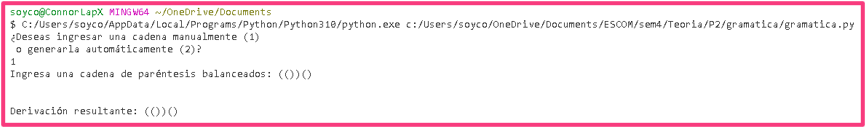
\includegraphics[width=4\linewidth]{Images/Cap1.png}
\end{minipage}
\caption{Inicio del programa en terminal.}
\label{fig:imagen}
\end{figure}
\newpage
\item Aquí se puede ver el archivo de salida de evaluacion.txt donde se pueden ver todos los pasos y reglas hechos por iteración.  Observar la Figura 2.2.\newline
\begin{figure}[h]
\begin{minipage}{0.3\textwidth}
    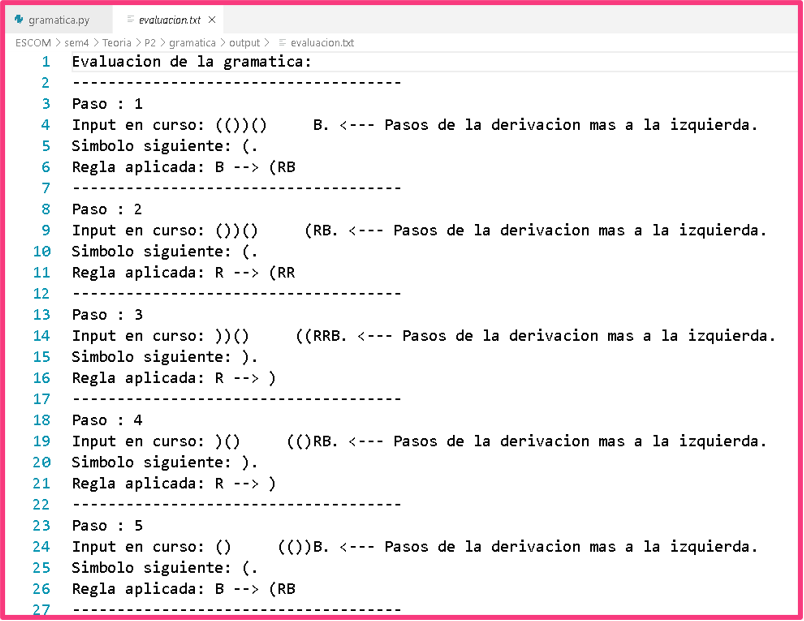
\includegraphics[width=4\linewidth]{Images/Cap2.png}
\end{minipage}
\caption{Primer parte de salida del archivo de evaluación.txt.}
\label{fig:imagen}
\end{figure}

\newpage
\item Aquí se puede ver el final del archivo de ejemplo que se ingresó como entrada, donde se pueden ver todos los pasos y reglas hechos por iteración. Observar la Figura 2.3.
\begin{figure}[h]
\begin{minipage}{0.3\textwidth}
    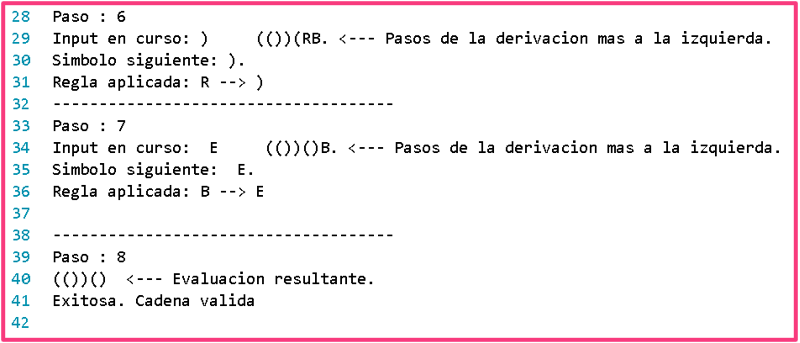
\includegraphics[width=4\linewidth]{Images/Cap3.png}
\end{minipage}
\caption{Segunda parte de salida del archivo de evaluación.txt.}
\label{fig:imagen}
\end{figure}

\newpage
\item Iniciamos nuevamente el programa, donde nos pide que introduzcamos una opción en el menú de inicio, la cadena que digitamos fue $"$)()()()()()()()()()()()()(()()()()()()()()()()()()()()(()()()()()()()()()()()()()()()()))$"$. Observar la Figura 2.4.
\begin{figure}[h]
%\begin{minipage}{0.3\textwidth}
    \begin{center}
    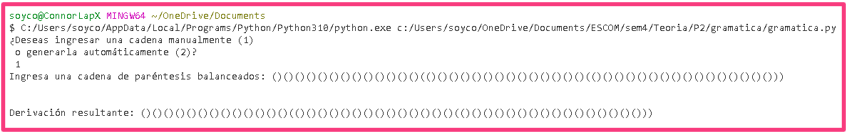
\includegraphics[width=1\linewidth]{Images/Cap4.png}
    \end{center}
%\end{minipage}
\caption{Visualización del programa en terminal.}
\label{fig:imagen}
\end{figure}

\newpage
\item Aquí se puede ver el final del archivo de ejemplo que se ingresó como entrada, donde se pueden ver todos los pasos y reglas hechos por iteración. Observar la figura 2.5.

\begin{figure}[h]
%\begin{minipage}{0.3\textwidth}
    \begin{center}
    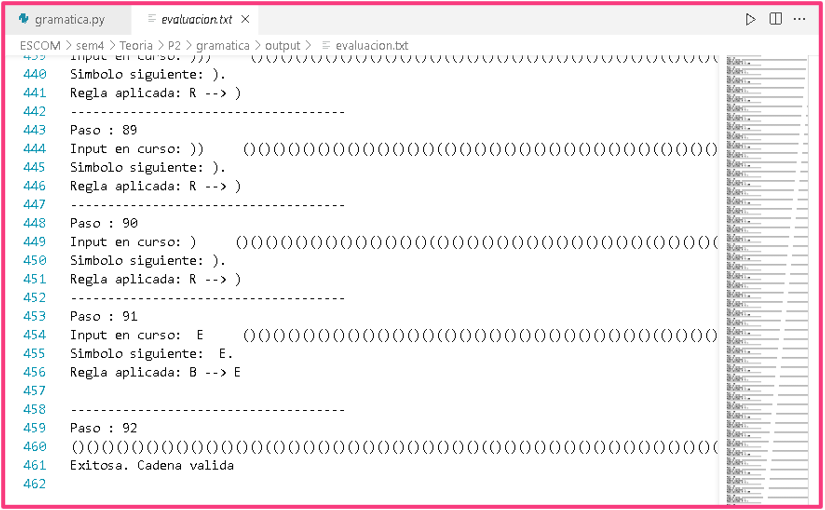
\includegraphics[width=1\linewidth]{Images/Cap5.png}
    \end{center}
%\end{minipage}
\caption{Visualización del archivo de salida evaluación.txt.}
\label{fig:imagen}
\end{figure}

\newpage
\item Iniciamos nuevamente el programa, donde nos pide que introduzcamos una opción en el menú de inicio, esta vez seleccionamos la opción aleatoria, para este ejemplo fue de tamaño 194. Observar la figura 2.6.

\begin{figure}[h]
%\begin{minipage}{0.3\textwidth}
    \begin{center}
    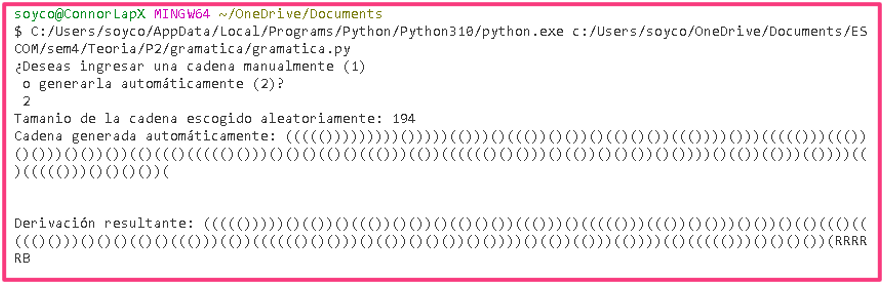
\includegraphics[width=1\linewidth]{Images/Cap6.png}
    \end{center}
%\end{minipage}
\caption{Visualización del programa en terminal.}
\label{fig:imagen}
\end{figure}
\newpage
\item Aquí se puede ver el final del archivo de ejemplo que se ingresó como entrada, donde se pueden ver todos los pasos y reglas hechos por iteración. Observar la figura 2.7.

\begin{figure}[h]
%\begin{minipage}{0.3\textwidth}
    \begin{center}
    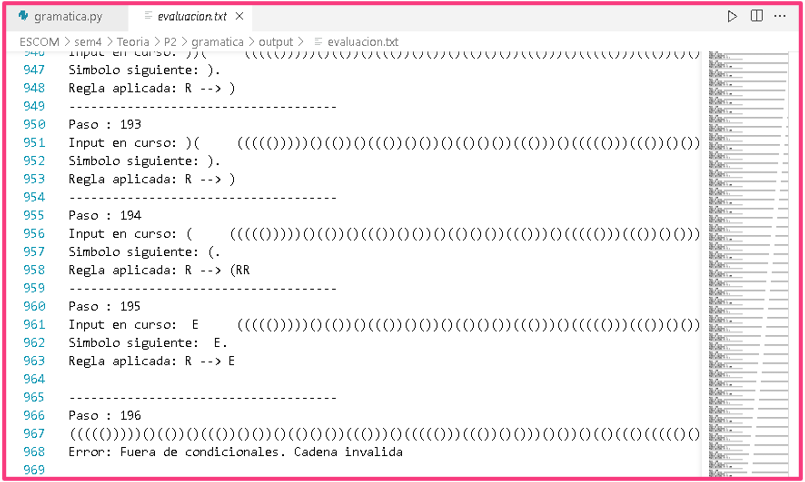
\includegraphics[width=1\linewidth]{Images/Cap7.png}
    \end{center}
%\end{minipage}
\caption{Visualización del archivo de salida evaluación.txt.}
\label{fig:imagen}
\end{figure}

\end{enumerate}
\chapter{Conclusión}

La conclusión de la resolución del programa es que se ha implementado un algoritmo para evaluar y derivar una cadena de paréntesis balanceados utilizando una gramática específica. El programa permite al usuario ingresar manualmente una cadena o generar una automáticamente.\newline

Durante la ejecución del programa, se lleva a cabo una evaluación paso a paso de la gramática, mostrando el input en curso, el símbolo siguiente, la regla aplicada y la evaluación resultante en cada paso. Esta información se registra en un archivo de texto para su posterior revisión.\newline

Además, el programa maneja los casos de cadenas de entrada inválidas o que no se pueden procesar correctamente, mostrando un mensaje de error correspondiente en tales casos.\newline

En general, la resolución del programa proporciona una forma interactiva y automatizada de evaluar y derivar cadenas de paréntesis balanceados según la gramática definida, brindando una herramienta útil para comprender y analizar este tipo de estructuras.\newline
\\

\section{Complejidades}
la complejidad del programa radica principalmente en el procesamiento de la gramática, que es lineal en función de la longitud de la cadena de entrada. Por lo tanto, podemos decir que la complejidad del programa en general es O(n), donde n es la longitud de la cadena de entrada.
\chapter{Bibliografias}
\begin{enumerate}
    \item Baron, N. S. (2015). Words Onscreen: The Fate of Reading in a Digital World. Oxford University Press.\newline
    \item García, M., & López, A. (2020). Parsing Algorithms for Balanced Parentheses Strings. Journal of Computer Science, 15(2), 245-259. \newline
    \item Smith, J. (2019). Introduction to Formal Languages and Automata Theory. Publisher.\newline
\end{enumerate}



%\textbf{Nota}: {\color{red}Revisar esta sugerencia de Segun:} %\href{https://github.com/INGEOTEC/RegionalEmbeddings}{FastText Word Embeddings for Spanish Language Variations} 


%[Objetivo: ]

\chapter{Anexos}
\lstset{
    language=C,
    basicstyle=\ttfamily\small\color{black},
    numbers=left,
    numberstyle=\tiny,
    stepnumber=1,
    numbersep=8pt,
    backgroundcolor=\color{white},
    showspaces=false,
    showstringspaces=false,
    showtabs=false,
    frame=single,
    rulecolor=\color{magenta},
    tabsize=2,
    captionpos=b,
    breaklines=true,
    breakatwhitespace=false,
    title=\lstname,
    escapeinside={\%*}{*)},
    keywordstyle=\color{blue},
    commentstyle=\color{red},
    stringstyle=\color{orange},
    morecomment=[l][\color{red}]{\#},
    otherkeywords={=,!,<,>,*,+,-,&,|,^,~},
    numbers=left,                   % Coloca los números de línea a la izquierda
    numberstyle=\tiny\color{black}, % Estilo de los números de línea
    stepnumber=1,    % Incremento en el que se muestran los números de línea
    numbersep=8pt
}
\section{Código LATEX de este documento}
Dirección GitHub:\url{}\newline
Dirección Overleaf:\url{https://www.overleaf.com/7893931279kkfrjsrcvgzx}\newline
\section{gramatica.py}
Se presenta el código implementado para la solución al problema con extensión .py . Donde es necesario tener importada la libreria random. \newline
\\
\begin{lstlisting}
#Teoria de la computacion
#Gramatica
#Alumno: Connor Urbano Mendoza

import random
#()()()()()()()()()()()()()(()()()()()()()()()()()()()()(()()()()()()()()()()()()()()()()))

# Función para generar automáticamente una cadena de paréntesis balanceados
def generate_balanced_parentheses(n):
    parentheses = ['(', ')']
    return ''.join(random.choice(parentheses) for _ in range(n))

def process_grammar(input_string):
    steps = "B"
    output = []
    i = 0
    posicion=0
    bandera=0
    contador=1
    with open('C:\\Users\\soyco\\OneDrive\\Documents\\ESCOM\\sem4\\Teoria\\P2\\gramatica\\output\\evaluacion.txt', 'w') as archivo:
        archivo.write("Evaluacion de la gramatica:"+ '\n')
        if i == len(input_string):
            return 'Invalid input string.'
        while 1:
            
            archivo.write("-------------------------------------"+ '\nPaso : '+str(contador)+'\n')
            if i >= 0 and i < len(input_string) and bandera==0:
                substring = input_string[i:]
                archivo.write("Input en curso: "+substring+ "     "+steps+". <--- Pasos de la derivacion mas a la izquierda.\n")
                archivo.write("Simbolo siguiente: "+input_string[i]+ '.\n')
            elif input_string=='ε':
                archivo.write("Input en curso:  E     "+steps+". <--- Pasos de la derivacion mas a la izquierda.\n")
                archivo.write("Simbolo siguiente:  E.\n")
            

            for symbol in steps:
                if symbol=="B":
                    LeftMostDerivation = "B"
                    break
                elif symbol=="R":
                    LeftMostDerivation = "R"
                    break
                posicion = posicion+1
            
            if LeftMostDerivation == 'B' and input_string[i] == '(':
                index = posicion
                steps = steps[:index] + '(RB' + steps[index+1:]  
                archivo.write("Regla aplicada: B --> (RB \n")
            elif LeftMostDerivation == 'B' and input_string[i] == '':
                index = posicion
                steps = steps[:index] + '' + steps[index+1:]  
                archivo.write("Regla aplicada: B --> E \n")
            elif LeftMostDerivation == 'R' and input_string[i] == ')':
                index = posicion
                steps = steps[:index] + ')' + steps[index+1:]  
                archivo.write("Regla aplicada: R --> ) \n")
            elif LeftMostDerivation == 'R' and input_string[i] == '(':
                index = posicion
                steps = steps[:index] + '(RR' + steps[index+1:]  
                archivo.write("Regla aplicada: R --> (RR \n")
            elif LeftMostDerivation == 'B' and input_string=='ε':
                index = posicion
                steps = steps[:index] + '' + steps[index+1:]
                archivo.write("Regla aplicada: B --> E \n")
                archivo.write("\n-------------------------------------"+ '\nPaso : '+str(contador+1)+'\n')
                archivo.write(steps+"  <--- Evaluacion resultante.\n")
                archivo.write("Exitosa. Cadena valida\n")
                return steps
            elif LeftMostDerivation == 'R' and input_string=='ε':
                archivo.write("Regla aplicada: R --> E \n")
                archivo.write("\n-------------------------------------"+ '\nPaso : '+str(contador+1)+'\n')
                archivo.write(steps+"  <--- Evaluacion resultante.\n")
                archivo.write("Error: Fuera de condicionales. Cadena invalida \n")
                return steps
            posicion=0 
            i =i+1
            contador=contador+1
            if i == len(input_string) or bandera==1:
                bandera=1
                i=0
                input_string='ε'



# Main
input_option = input("¿Deseas ingresar una cadena manualmente (1)\n o generarla automáticamente (2)?\n ")

if input_option == '1':
    input_string = input("Ingresa una cadena de paréntesis balanceados: ")
elif input_option == '2':
    numero=random.randint(1, 1000)
    print("Tamanio de la cadena escogido aleatoriamente: "+str(numero))
    input_string = generate_balanced_parentheses(numero)
    print("Cadena generada automáticamente:", input_string)
else:
    print("Opción inválida. El programa se cerrará.")
    exit()

derivation = process_grammar(input_string)
print("\n\nDerivación resultante:", derivation)

\end{lstlisting}


%\bibliographystyle{apacite}
%\bibliography{References/predoc.bib}

\backmatter%@sglvgdor


\end{document}
